\section{Locating the Consistency Boundary (RQ1)}
\label{sec:diagnosis}
\subsection{A repair and a regression under the same intervention}
An RTX intervention changes target continuation from UB2 to UB1 while retaining the registered prefill, draft and caller grouping. On 19 exposed HumanEval tasks, the source-bound predictor reproduces both native conditions on all 57 repeated complete arrays. Nevertheless, HumanEval/15 repairs, /25 regresses, and /18 remains divergent. Reference agreement stays at 51/57 in both conditions. An unchanged aggregate therefore hides opposing task-level effects; it is not an all-task no-op.

A separately selected 24-task MBPP panel has 72/72 prediction/native agreement in each condition but only 66/72 reference agreement. One persistent failure, MBPP/304, changes token 488 to 481 at zero-based position 33 while remaining a 47-ID divergent response. Prediction fidelity, response change, and reference restoration are three different outcomes. The continuation intervention alone fails the intended recovery-without-regression objective.

\subsection{Natural donor state crossed with the current call}
Four exposed HumanEval probes are examined at frozen natural cuts. Across repetitions, 24 donors support 48 state/current-path forks and 24 own-path shams. Donors retain actual pending state, cache positions and sampler behavior. Own-path decisions reproduce the original execution, and the original context remains unchanged after forking. Auxiliary short continuations and their 1,278 forwards are diagnostic work, not a performance panel.

Figure~\ref{fig:cross} shows discriminating IDs. At /15, with 13 committed tokens, changing the current UB2/UB1 recipe changes the third submitted decision from 9147 to 4199 under either donor. At /25, with four committed tokens, only the N1 donor/current-UB1 cell changes the submitted decision. That cell produces IDs 271,750,8168 rather than 1406. The effect is an interaction, not an explanation based only on donor state. At the selected /18 and /31 cuts, both recipes and donors preserve the discrete decision. These nulls are local and do not establish trajectory-wide invariance.

\begin{figure*}[t]
\centering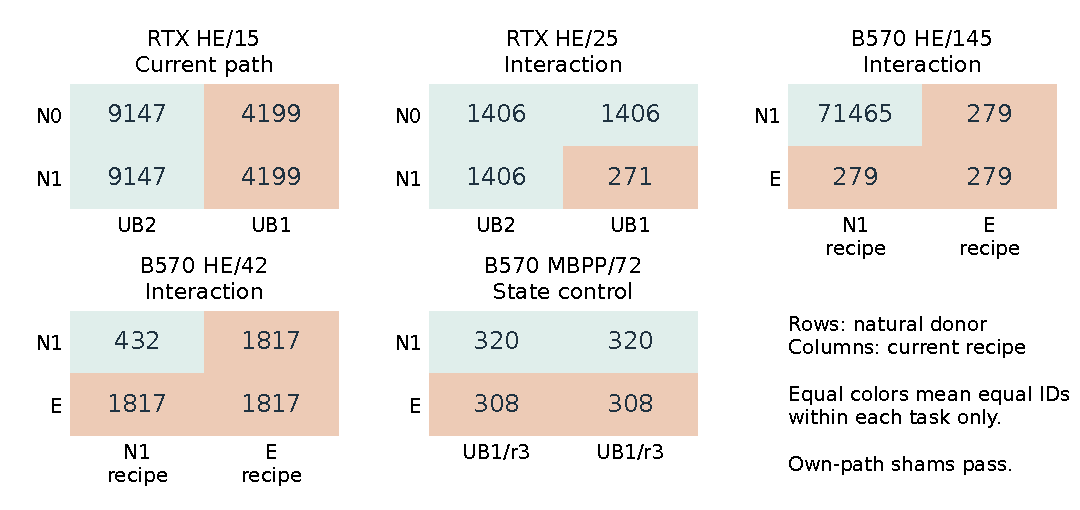
\includegraphics[width=\linewidth]{figures/figure_2_natural_crosses.pdf}
\caption{Source-derived RTX and B570 natural-state crosses. Rows are donors and columns current recipes. Cell labels are the discriminating sampled/argmax ID; colors group equal IDs within each task only. RTX /15 shows a current-path effect and /25 an interaction. B570 /145 and /42 cross N1 (UB1/reservation3) with E (UB2/reservation2); /72 has identical UB1/reservation3 current columns and is a state control. All repetitions reproduce the displayed local patterns.}
\label{fig:cross}
\end{figure*}

The RTX donor comparison also distinguishes logical tensor equality from file hashes. All 12 prompt-KV pair comparisons agree, while 70 of 72 generated-prefix K/V tensor comparisons differ; tested first-layer logical K/V remain equal. This supports examining state formation and attention-related execution, but does not identify attention as the sole cause. In particular, the discriminating /15 bonus row is itself a single-token microbatch under both histories. The final row's nominal shape cannot explain the entire effect without considering its inputs and preceding work.

\subsection{One unchanged block does not certify the remaining trajectory}
A separate B570 experiment starts both branches from the same live fork state, with byte-checked KV, and intervenes on one target verification block, comparing UB1 with UB128. The frozen checkpoint is the first eligible block reached after at least 64 committed IDs. Twenty-four reserved prompts with three repetitions provide 72 eligible forks. All 72 paired raw score records change, yet top-1 IDs and actual immediate decisions do not: zero of 72 executions and zero of 24 tasks show an immediate decision difference across 195 paired decision events.

Continuing under the frozen policy gives a different result. Complete downstream committed-ID trajectories change in 18 of 72 executions, corresponding to six of 24 tasks. Later alternate target blocks retain UB128 and proposals evolve, so the secondary result is not an isolated one-block perturbation followed by restored execution. The score effect and delayed trajectory effect coexist with an immediate discrete null. The intervention's primary sampled-block result therefore cannot be relabeled either an immediate decision effect or a whole-output no-effect result. Its engineering implication is direct: qualification must continue beyond a locally unchanged acceptance decision. Neither logit movement nor one-step agreement replaces complete registered-output checking.

\subsection{B570 crosses identify a whole-recipe boundary}
Later B570 natural-state crosses cover three tasks in two contexts, with 12 complete own-path shams and 24 auxiliary target cells. Restored states are checked for byte consistency, sequence-zero ownership and logical position. Figure~\ref{fig:cross} includes the selected argmax matrices. HumanEval/145 has $[(71465,279),(279,279)]$ at prefix 56, and /42 has $[(432,1817),(1817,1817)]$ at prefix 73. Both are local interactions. MBPP/72 has $[(320,320),(308,308)]$ at prefix 40: donor state changes the decision while the current columns are the same UB1/output-reservation-3 recipe.

For the HumanEval crosses, the current recipes change microbatch and output reservation together. The appropriate causal factor is the current whole recipe, not UB alone. The repeated cases are three tasks, not six independent task discoveries. Full counterfactual continuations from each cross cell are unavailable; the subsequent candidate has a separate native endpoint qualification panel. The greedy sampler contract is supported by live history, clone metadata and shams, while opaque sampler bytes and general stochastic-state restoration remain unavailable.

These observations carry the same experimental question across CUDA and Vulkan without transferring the same repair. Some boundaries are path-sensitive, others state-sensitive or interactive. A runtime designer cannot infer the required control placement from committed-prefix equality or a single margin alone.

\subsection{Prediction and simple execution constrain added machinery}
Earlier prediction studies remain useful but answer a narrower question. B570 prospective prediction matches 72/72 native arrays on a reserved 24-task cohort even when reference agreement is 60/72. RTX's first target-only batched-path predictor reaches 24/36, below its frozen 36/36 gate, so that study performs zero reserved inference. A later independent-proposal replay implementation obtains H2/native and reference-only/native prediction agreement of 72/72, with reference agreement still 60/72. The first implementation's missing interface is resolved by that later study; neither result makes replay a cheap online repair.

A fresh ordinary target-only bridge provides an especially strong simple alternative. On the 19 RTX tasks, draft-free $U_2$ reproduces all 57 intervention $N_1$ arrays and strict stop boundaries without a draft, transplant, proposal tape or answer. It reproduces both /15's repair and /25's regression. This is output equivalence, not demonstrated equivalence of unavailable live logits/KV or a speed result.

Finally, retrospective selector feasibility finds no additional supported capability: RTX direct enumeration and proxy screening both abstain at 114 post-common-acquisition record equivalents; B570 needs 72 for direct verification and 144 for proxy screening. Unknown counterfactuals remain unknown. These costs are acquisition equivalents, not measured latency. Together, the results answer RQ1 with local state/path evidence while rejecting the shortcut from an accurate reproducer to a useful automatic repair selector.
